%======================== 2. PROBLEM 1: SEARCH, ALIGN, BRAKE ===================
\isec{\faCrosshairs}{Problem 1: Visual Search, In-Place Centering and Standoff Guard}

\isub{\faCamera}{(i) Downward camera setup}
\label{sec:arm}

\lead{Why the assignment pose tilts the camera down.}
\begin{itemize}
  \item The EP arm is a two-servo parallel-link arm. The SDK arm command $(X,Y)$ is the end effector position in the
        arm plane: $X$ forward reach, $Y$ height, in millimeters.
  \item The camera bracket is fixed to an arm link, so its pitch is not set independently: it follows the joint
        angles that the arm needs to reach $(X,Y)$.
  \item Lowering the end effector ($Y=30$\,mm, close to the bottom of the workspace) with a short reach
        ($X=105$\,mm, close to the retracted end) rotates that link forward and down, so the optical axis pitches below
        the horizon and the floor in front of the robot enters the image. With a level camera the floor tags would sit
        in the lower edge of the image or below it.
  \item On a stock EP the front ToF sensor sits low on the chassis front and looks forward horizontally. With a short
        reach the gripper stays above and behind the sensor face, so the beam leaves the robot unobstructed while the
        camera looks over it at the floor. The tags lie flat, so the beam passes over them and stays free to detect real
        obstacles ahead.
\end{itemize}

\begin{warnbox}
\small\textbf{\color{warn}\faExclamationTriangle\ Deviation on this robot: the assignment pose collides with the ToF sensor}
\begin{itemize}
  \item On this robot the front ToF sensor is mounted on the top front rail, directly under the gripper
        (Figure~\ref{fig:photos}). It could not be moved to another mount.
  \item Commanding $X=105$\,mm, $Y=30$\,mm drives the gripper into the sensor: with no goal active the arm kept moving,
        \code{arm_position} $(x,z)$ going from (0.136, 0.077) to (0.122, 0.050)\,m in 3\,s and then from (0.138, 0.087) to
        (0.127, 0.057)\,m, hunting while it pushed on the sensor (\code{notes/lab_log.md}, 00:02 to 00:05). The stall guard in \code{tag_detector} (optional \code{init_arm}) and
        \code{tools/arm_step.py} cancel such a move and hold the arm where it stopped.
  \item \textbf{Adopted solution:} the arm was set by hand about 2\,cm above the ToF sensor. The driver reported
        \code{arm_position} $x=0.1230$\,m, $z=0.0670$\,m (39 samples, std 0.0\,mm, \code{notes/lab_log.md}, 01:10),
        saved in \code{config/robot.yaml}. The camera is still pitched
        down (by $5.3^\circ$, measured from the floor tag, Section~\ref{sec:geom}) and the ToF beam is clear.
  \item \textbf{Arm guard:} the camera calibration is valid only at this pose, so \code{flatness_planner} refuses to
        start until \code{arm_position} is within 6\,mm of the saved pose and brakes for good (ARRIVED, reason
        ``arm moved'') if the arm drifts more than 6\,mm during a mission.
  \item The detector logs confirm that the camera pitch follows the arm: earlier hand-set poses in the same session gave
        $15.9^\circ$, $6.3$ to $6.6^\circ$, $7.9$ to $8.0^\circ$ and $5.5$ to $5.7^\circ$ downward pitch, all measured from the
        floor tag.
\end{itemize}
\end{warnbox}

\begin{figure}[H]
\centering
\begin{subfigure}{0.31\linewidth}\centering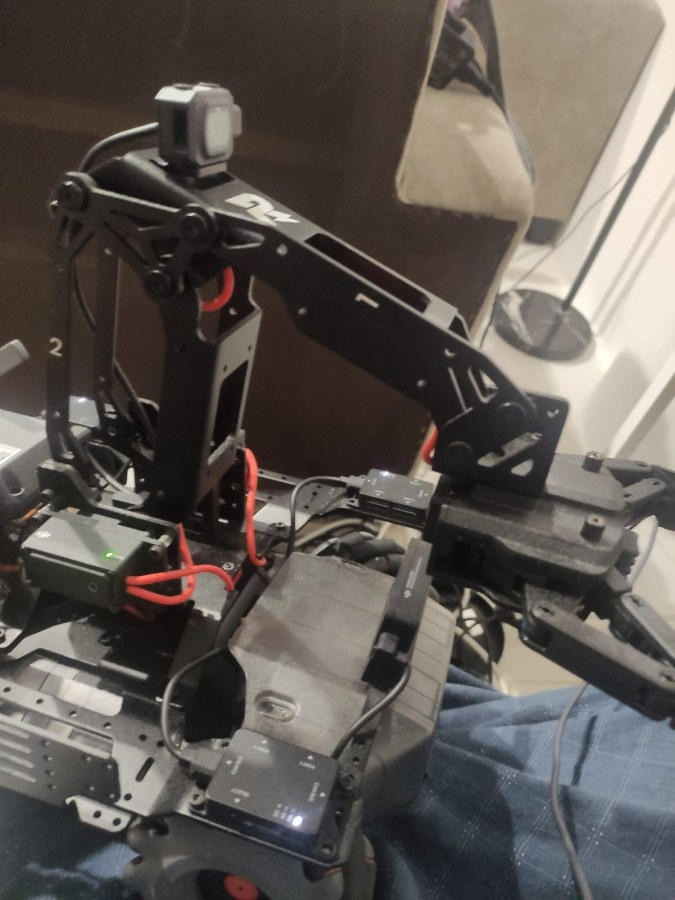
\includegraphics[height=6.2cm]{figures/photo_arm_side.jpg}
\caption{Side view: camera on the arm link, gripper at the front.}\end{subfigure}\hfill
\begin{subfigure}{0.31\linewidth}\centering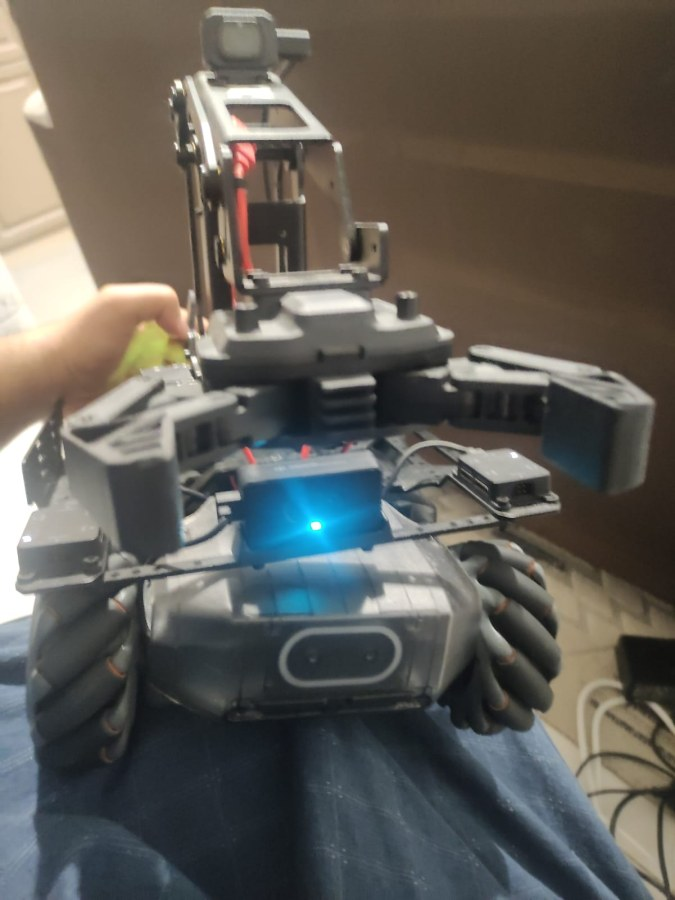
\includegraphics[height=6.2cm]{figures/photo_front_tof.jpg}
\caption{Front view: the ToF sensor (blue light) on the top front rail, under the gripper.}\end{subfigure}\hfill
\begin{subfigure}{0.31\linewidth}\centering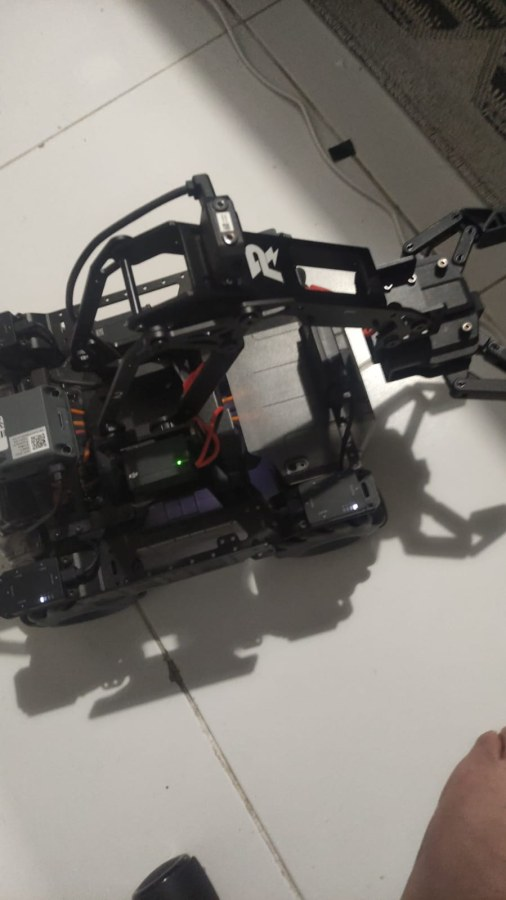
\includegraphics[height=6.2cm]{figures/photo_top_view.jpg}
\caption{Top view: arm and gripper over the front rail.}\end{subfigure}
\caption{Arm and ToF arrangement of the robot used (photos by the student). The low end effector pose of the
assignment would press the gripper onto the ToF sensor, so the arm was set by hand about 2\,cm above it.}
\label{fig:photos}
\end{figure}

\isub{\faRulerCombined}{Camera geometry: ground range, not slant range}
\label{sec:geom}
\label{sec:tf}

\begin{figure}[H]
\centering
\begin{tikzpicture}[x=6.6cm,y=6.6cm,font=\small]
  % floor
  \fill[pattern=north east lines,pattern color=muted!50] (-0.42,-0.025) rectangle (1.6,0);
  \draw[ink,thick] (-0.42,0) -- (1.6,0);
  % blind zone on the floor
  \fill[accred!18] (0.162,0) rectangle (0.445,0.018);
  % chassis (schematic)
  \draw[ink,fill=muted!25,rounded corners=2pt] (-0.30,0.05) rectangle (0.162,0.17);
  \foreach \x in {-0.20,0.07} \draw[ink,fill=ink!70] (\x,0.05) circle (0.05);
  \node[font=\scriptsize] at (-0.07,0.11) {chassis (schematic)};
  % arm post and camera
  \draw[ink,line width=2pt] (-0.06,0.17) -- (-0.02,0.30) -- (0,0.313);
  \draw[ink,fill=ink] (-0.022,0.300) rectangle (0.022,0.326);
  % ToF beam
  \fill[accorange] (0.150,0.185) rectangle (0.168,0.205);
  \draw[accorange,thick,-{Latex[length=2mm]}] (0.168,0.195) -- (0.85,0.195)
     node[right,font=\scriptsize,align=left]{front ToF beam (horizontal):\\passes over a flat tag, no echo};
  % optical axis and lower FOV edge
  \draw[kfupm,thick,dash pattern=on 5pt off 2pt] (0,0.313) -- ($(0,0.313)+(-5.3:1.6)$) node[above left,font=\scriptsize,text=kfupmdark]{optical axis, $\varphi=5.3^\circ$ down};
  \draw[kfupm] (0,0.313) -- (0.445,0);
  \fill[kfupm,opacity=0.07] (0,0.313) -- (0.445,0) -- (1.6,0) -- (1.6,0.165) -- cycle;
  \node[font=\scriptsize,text=kfupmdark,align=left] at (0.62,0.07) {lower image edge\\$35.1^\circ$ below horizon};
  % tag at the standoff and slant vs ground range
  \fill[black] (0.362-0.0775,0) rectangle (0.362+0.0775,0.008);
  \draw[accblue,thick] (0,0.313) -- (0.362,0.004);
  \node[font=\scriptsize,text=accblue,align=left,anchor=west] at (0.22,0.30) {slant range 0.479\,m};
  \draw[accblue,->] (0.22,0.29) -- (0.17,0.17);
  % dimensions
  \draw[|<->|,muted] (-0.36,0) -- node[left,font=\scriptsize,text=ink,align=right]{$h=0.313$\,m\\(from tag)} (-0.36,0.313);
  \draw[dotted,muted] (-0.36,0.313) -- (0,0.313);
  \draw[|<->|,muted] (0,-0.07) -- node[below,font=\scriptsize,text=ink]{0.162\,m} (0.162,-0.07);
  \draw[|<->|,accblue] (0,-0.16) -- node[below,font=\scriptsize,text=accblue]{ground distance 0.362\,m} (0.362,-0.16);
  \draw[|<->|,accred] (0.162,-0.07) -- node[below,font=\scriptsize,text=accred]{blind 0.283\,m} (0.445,-0.07);
  \draw[|<->|,kfupmdark] (0.162,0.36) -- node[above,font=\scriptsize,text=kfupmdark]{standoff 0.20\,m} (0.362,0.36);
  \draw[dotted,muted] (0.162,0.36) -- (0.162,0.17); \draw[dotted,muted] (0.362,0.36) -- (0.362,0.01);
  \draw[dotted,muted] (0,-0.17) -- (0,0.30);
  \node[font=\scriptsize,anchor=west] at (1.0,-0.07) {T3 at the 20\,cm standoff (black bar)};
  \node[font=\scriptsize,anchor=west,text=accred] at (1.0,-0.13) {red floor band: no floor point visible};
\end{tikzpicture}
\caption{Side view of the camera geometry at the arm pose used (to scale, chassis schematic). Distances are
measured from the chassis front. At the standoff the tag is already below the image, and its slant range from the
camera is 0.479\,m.}
\label{fig:geom}
\end{figure}

\lead{The driver's arm TF is wrong for this arm.} The TF chain \code{base_link} $\rightarrow$
\code{camera_optical_link} published by the driver put the optical axis $18^\circ$ \emph{up} after the A2 arm move and
$22^\circ$ up with the arm resting on the ToF sensor, while the floor tag showed the same camera $15.9^\circ$
\emph{down}; with the $18^\circ$ TF the floor tag even came out 0.378\,m above the camera (\code{notes/lab_log.md}). The detector therefore does not use TF
(\code{extrinsics: tag}); it measures the camera pose from the floor tag itself.

\lead{Camera height and pitch from one floor tag} (\code{camera_from_floor_tag} in \code{geometry.py}).
pupil-apriltags returns the tag pose $(\mathbf R,\mathbf t)$ in the optical frame ($x$ right, $y$ down, $z$ forward).
A tag lying flat has its normal along the floor normal, so with $\mathbf n=\pm\mathbf R_{:,3}$ oriented toward the camera:
\begin{equation}
h=-\mathbf n^{T}\mathbf t,\qquad \varphi=\arcsin(-n_z),\qquad \text{roll}=\operatorname{atan2}(n_x,\,-n_y).
\end{equation}
No arm model or TF is needed. At the final arm pose this gave $h\approx0.313$\,m and $\varphi=5.3^\circ$ (roll within
$\pm0.4^\circ$), now fixed parameters of the detector.

\lead{Ground range and bearing} (\code{camera_to_level}). The tag center $\mathbf p=(x,y,z)$ is rotated into a level
frame at the camera, and the calibrated offset to the chassis front is applied:
\begin{equation}
\begin{aligned}
p_{fwd}&=z\cos\varphi-y\sin\varphi, \qquad p_{left}=-x,\\
d&=s\,p_{fwd}+o,\quad s=1.0,\ o=-0.162\text{\,m},\qquad \theta=\operatorname{atan2}(p_{left},\,p_{fwd}).
\end{aligned}
\end{equation}

\begin{bluebox}{\faRulerHorizontal\ \ Why the slant range must not be used for the brake}
\small
\begin{itemize}
  \item The straight-line range $\|\mathbf p\|$ contains the camera height. At the 20\,cm standoff the ground distance
        from the camera is $0.20+0.162=0.362$\,m but the slant range is $\sqrt{0.362^2+0.313^2}=0.479$\,m.
  \item Using the slant range with the same front offset would read $d=0.317$\,m at the standoff: the robot would
        brake about 11.7\,cm late, at roughly 8\,cm from the tag. The offline test
        \code{test_slant_range_overshoots_standoff} checks the same effect for the note example (0.32\,m read at 0.20\,m).
  \item The bearing error of the tilted camera is small; the range error is not.
\end{itemize}
\end{bluebox}

\isub{\faEye}{Range calibration and detection range}
\begin{itemize}
  \item \textbf{Tag:} printed T3 measured with a ruler: 155\,mm black edge (printer scale about 98\,\%), so
        \code{tag_size} $=0.155$\,m. Camera at 720p ($f_x=628.6$, $f_y=625.8$\,px).
  \item \textbf{Calibration:} T3 at tape distances from the chassis front; \code{tools/tag_range_probe.py} averaged 5\,s of
        detections. Rows 3 to 6 of \code{data/calibration/tag_range.csv} (1.20, 1.50, 0.60, 1.00\,m, 01:00:44 to
        01:07:34) were taken at the final arm pose, after the router-mode restart and before the pose was saved at 01:10;
        rows 1 and 2 belong to an earlier pose and are not used.
  \item \textbf{Model:} with the horizontal camera distance re-derived from the logged slant range and a camera height of
        0.310\,m, the offsets (tape minus camera) are $-0.0991$, $-0.1621$, $-0.1675$ and $-0.1619$\,m. Their median,
        $-0.1620$\,m, is the configured $o$ with scale $1.0$. A least-squares line gives scale 1.0176 and offset
        $-0.1692$\,m, pulled by the 1.20\,m point. With $o=-0.162$\,m the estimate minus tape is $+0.1$, $+5.5$ and
        $-0.1$\,mm at 1.50, 0.60 and 1.00\,m; the 1.20\,m point is an outlier at $-63$\,mm, most likely a misplaced
        tag, and the median is insensitive to it.
  \item \textbf{Real range limit:} at the final pose T3 was detected at 1.50\,m at 3.8 detections/s and at 0.6 to
        1.0\,m at 13.6 to 14.8 detections/s; at 1.80\,m the probe printed ``NOT DETECTED in 8\,s'' while the detector
        processed about 14 frames/s (\code{notes/lab_log.md}, 01:03; the probe writes no CSV row on a miss).
        The range limit of this 155\,mm tag lies between 1.5 and 1.8\,m, so all floor runs start at 1.50\,m
        (Figure~\ref{fig:range}).
\end{itemize}

\begin{figure}[H]
\centering
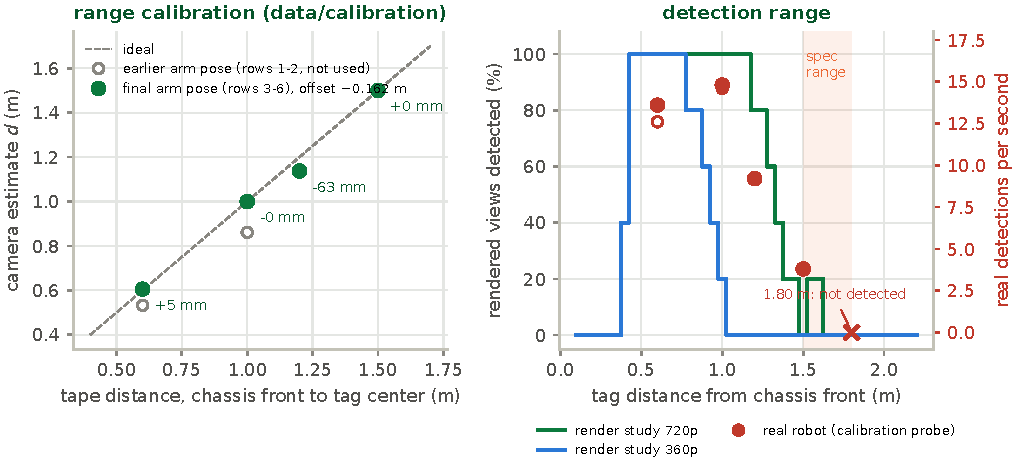
\includegraphics[width=\linewidth]{figures/p1_range.pdf}
\caption{Left: camera range estimate against the tape distance. Right: offline render study (real T3 bitmap on the
floor, calibrated 720p and 360p cameras at $h=0.313$\,m, $\varphi=5.3^\circ$, five in-plane tag rotations per
distance) and real detection rates. The render study is an ideal-image upper bound: at 720p every rotation is
detected from 0.45 to 1.15\,m and some up to 1.60\,m; 360p would stop near 1.0\,m.}
\label{fig:range}
\end{figure}

\isub{\faSyncAlt}{(ii) Search and centering finite state machine}
\label{sec:fsm}
The planner runs the state machine of Figure~\ref{fig:fsm} with the parameters of Table~\ref{tab:fsm}; the brake
conditions are detailed in Section~\ref{sec:brake}.

\begin{figure}[H]
\centering
\begin{tikzpicture}[font=\small]
  \node[stnode=SEARCHING] (S) at (0,0) {\textbf{\textcolor{cSEARCHING}{SEARCHING}}\\[1pt]\footnotesize
     $v=0$\\$\omega=\pm0.30$\,rad/s toward the\\side where T3 was last seen};
  \node[stnode=ALIGNING] (A) at (8.4,0) {\textbf{\textcolor{cALIGNING}{ALIGNING}}\\[1pt]\footnotesize
     $v=0$\\$\omega=1.0\,\theta$, $0.10\le|\omega|\le0.30$\,rad/s};
  \node[stnode=CHASING] (C) at (8.4,-4.0) {\textbf{\textcolor{cCHASING}{CHASING}}\\[1pt]\footnotesize
     $v=\dot x_{ref}(t)$ (cubic plan)\\$\omega=\omega_{ref}+0.8\,\theta$, $|\omega|\le0.30$};
  \node[stnode=ARRIVED] (R) at (0,-4.0) {\textbf{\textcolor{cARRIVED}{ARRIVED}}\\[1pt]\footnotesize
     active brake\\$v=0$, $\omega=0$ held};
  \draw[tr] ([yshift=4mm]S.east) -- node[trl,above=1pt]{T3 detected (age $\le0.45$\,s)} ([yshift=4mm]A.west);
  \draw[tr] ([yshift=-4mm]A.west) -- node[trl,below=1pt]{T3 hidden $>0.45$\,s} ([yshift=-4mm]S.east);
  \draw[tr] (A) -- node[trl,right=2pt,align=left]{$|\theta|\le0.18$\,rad on 3 consecutive\\detections: fix $d_0$, solve\\
     the cubic, start the clock} (C);
  \draw[tr] (C.north west) -- node[trl,sloped,above=1pt]{hidden $>2.0$\,s and $>0.25$\,m to go} (S.south east);
  \draw[tr,color=cARRIVED] (C) -- node[trl,above=2pt,align=center,text=ink,font=\scriptsize]{camera $d\le0.20$ \textbf{or} ToF $\le0.20$\\
     \textbf{or} odom.\ $\ge d_0-0.20$ \textbf{or} $t\ge T$} (R);
  \draw[tr,color=cARRIVED] (R.south west) .. controls +(-1.0,-0.9) and +(1.0,-0.9) .. (R.south east)
     node[pos=0.5,below,font=\scriptsize,text=ink]{every tick};
  \draw[tr,color=muted] (-2.3,1.35) node[above,font=\scriptsize,text=ink,align=center]{start: arm within\\6\,mm of saved pose} -- (S.north west);
  \node[draw=alert,dashed,rounded corners=3pt,font=\scriptsize,align=left,text width=4.1cm,fill=alert!4] at (4.2,-5.7)
     {\faShieldAlt\ any state: arm moved $>6$\,mm $\rightarrow$ ARRIVED. Every exit path (end, Ctrl+C, exception)
      sends zero velocity.};
\end{tikzpicture}
\caption{Supervisory state machine of \code{mission.py}, run by \code{flatness_planner} at 20\,Hz.
$\theta$ is the tag bearing ($+$ left), $d$ the ground range from the chassis front.}
\label{fig:fsm}
\end{figure}

\begin{table}[H]
\centering\small
\rowcolors{2}{kfupmlight}{white}
\begin{tabularx}{\linewidth}{@{}l c >{\raggedright\arraybackslash}X@{}}
\rowcolor{kfupm}\hd{Parameter} & \hd{Value} & \hd{Role}\\
\code{lost_timeout} & 0.45\,s & tag counts as hidden after this age (assignment value) in SEARCHING and ALIGNING\\
\code{search_rate} & 0.30\,rad/s & in-place sweep, sign from the last seen bearing (default CCW)\\
\code{align_tol}, \code{align_settle} & 0.18\,rad, 3 & centered when $|\theta|\le0.18$ on 3 consecutive detections\\
\code{align_gain}, min, max & 1.0, 0.10, 0.30\,rad/s & proportional turn; the minimum overcomes the chassis dead band\\
\code{chase_gain} & 0.8\,rad/s per rad & bearing correction added to the plan's $\omega_{ref}=0$ while T3 is visible\\
\code{chase_lost_timeout} & 2.0\,s & dropouts tolerated while chasing (about 4 detections/s at 1.5\,m)\\
\code{blind_zone} & 0.25\,m & remaining planned distance below which losing T3 is expected and ignored\\
\code{standoff}, \code{tof_brake} & 0.20\,m, 0.20\,m & brake thresholds; ToF readings below 0.02\,m are ignored\\
\end{tabularx}
\caption{State machine parameters (\code{MissionParams} in \code{mission.py}).}
\label{tab:fsm}
\end{table}

\begin{keybox}{\faCompass\ \ Why the robot aligns in place before translating}
\small
\begin{itemize}
  \item \textbf{The plan is only valid for a tag straight ahead.} The flat output is built in the robot frame at the
        chase start with $y(t)\equiv0$, a straight line along body $+X$. If the tag sits at bearing $\theta_0$, the
        plan ends $d_0\sin\theta_0$ to the side of it: 0.23\,m for $\theta_0=0.18$\,rad at $d_0=1.27$\,m, and
        0.95\,m for the $43.7^\circ$ (at $d=1.37$\,m) at which T3 first appeared in the final run. Centering first makes the straight
        flat output (zero curvature, $\omega_{ref}=0$) the right path; the remaining small error is removed by the bearing
        feedback.
  \item \textbf{It keeps the tag in view.} The half field of view is about $45^\circ$ and T3 is detected only up to about
        1.5\,m, with 3.8 detections/s at 1.5\,m. A turn while translating moves the tag across the image by rotation
        and parallax at once, so a tag near the edge leaves the view; motion blur also lowers the detection rate at
        the range limit. In-place rotation keeps the distance constant, so the tag stays at a detectable range while
        it moves to the image center, where the pose estimate is best.
  \item \textbf{It prevents trajectory drift.} Pure rotation and pure translation are the two motions the chassis
        tracks best; combined turning and driving adds roller slip and heading error to the odometry. The odometry
        stop criterion (straight distance $\ge d_0-0.20$) and the plan time $T$ both assume a straight path.
  \item \textbf{$d_0$ is measured at its best.} $d_0$ fixes the goal and the horizon $T$. It is taken when the tag is
        centered and the robot is still, not from a moving, off-center view.
\end{itemize}
\end{keybox}

\isub{\faStopCircle}{(iii) Standoff braking}
\label{sec:brake}
CHASING switches to ARRIVED on the first of four conditions, checked every 50\,ms tick before a command is sent:
\begin{enumerate}
  \item \textbf{camera} $d\le0.20$\,m while the tag is visible (assignment requirement),
  \item \textbf{front ToF} range $\le0.20$\,m (assignment requirement; readings $\le0.02$\,m are treated as no echo),
  \item \textbf{odometry}: straight distance from the chase start $\ge d_0-0.20$,
  \item \textbf{plan time}: $t\ge T$; the plan itself ends at $\dot x(T)=0$, so this is a smooth stop.
\end{enumerate}
ARRIVED then sends $v=0$, $\omega=0$ on every tick, keeps logging (3\,s of zero rows), and the node sends zero velocity
again on shutdown, on Ctrl+C and on exceptions.

\begin{warnbox}
\small\textbf{\color{warn}\faEyeSlash\ The camera cannot see the tag at the standoff}
\begin{itemize}
  \item With $\varphi=5.3^\circ$ and a $29.8^\circ$ half field of view below the axis, the lowest image row meets the floor
        0.283\,m from the chassis front; the whole 155\,mm tag is in view only beyond about 0.36\,m
        (Figure~\ref{fig:geom}). The last detections of the three floor runs were at 0.391, 0.397 and 0.400\,m.
  \item Condition 1 is implemented as specified, but at this arm pose it cannot fire; it would with the steeper
        assignment pose. A flat floor tag gives no ToF echo (the ToF read 0.382 to 0.865\,m during the final run), so
        condition 2 is the obstacle guard.
  \item The final approach is therefore carried by the plan and the odometry (conditions 3 and 4). Losing the tag
        within the last \code{blind_zone} of the plan does not abort the chase. All three floor runs stopped on these
        conditions and measured 21, 20 and 20\,cm with the tape (Section~\ref{sec:results}).
\end{itemize}
\end{warnbox}

\isub{\faFilm}{Implementation hint: preventing video stalls}
The hint targets a script that pulls frames with \code{cap.grab()} from an FFmpeg decoder: if frames are grabbed
faster than the decoder recycles its buffers, \code{av_frame_get_buffer} runs out of memory and the stream stalls.
This package has no grab loop, and it handles the same problem as follows:
\begin{itemize}
  \item \textbf{The driver owns the decoder.} \code{robomaster_ros} decodes the H.264 stream and publishes raw
        \code{camera/image_color}. The detector never holds a decoder buffer, it only receives ROS messages.
        (PyAV is not installed, which the driver reports as ``FFmpeg not available''; raw images still publish.)
  \item \textbf{Newest frame only.} The image callback stores only the latest message; a 15\,Hz timer takes it and
        clears the slot. A slow detection drops frames instead of queuing them, which is what the sleep between
        \code{grab()} calls achieves in the hint. During the final run the detector processed 13.0 to 14.4 frames/s.
  \item \textbf{Watchdog.} If no image arrives for 2\,s, the detector re-creates its camera subscriptions, which recovers
        the stream after a driver reconnect (logged as ``No camera image for 2.4\,s: re-subscribing'').
\end{itemize}
